
\bigskip

On veut fabriquer un escalier en bois de hauteur \np[cm]{272}.

La figure ci-dessous représente une vue de profil de cet escalier.

La hauteur d'une marche est de \np[cm]{17}.

La profondeur d'une marche pour poser le pied mesure \np[cm]{27}.

\begin{center}
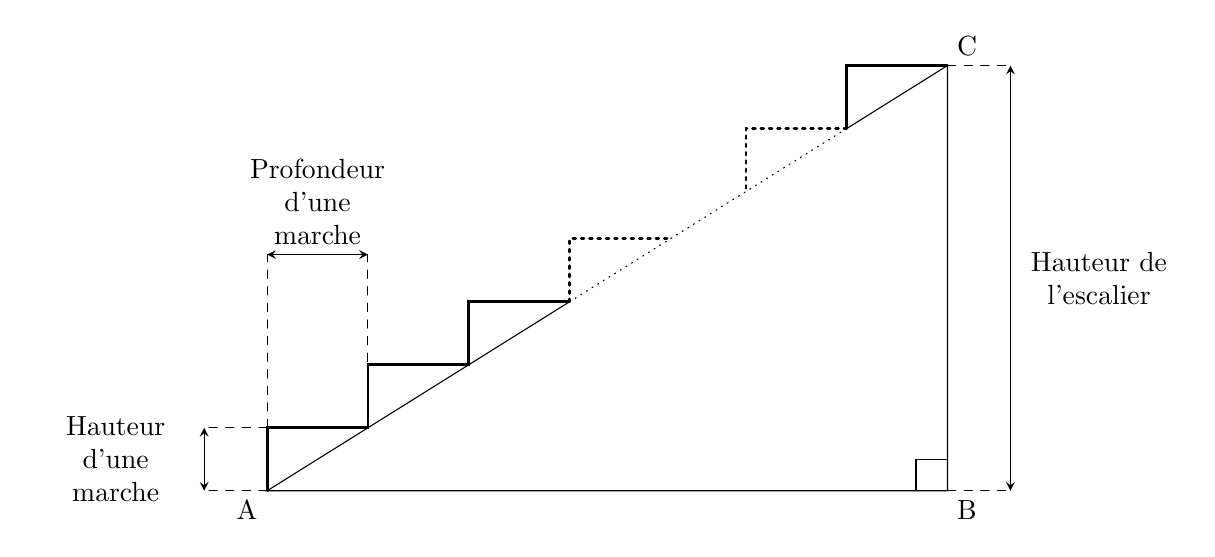
\begin{tikzpicture}[line cap = round,>=stealth,x =8mm]
        \draw[dashed] (0,0)--(-1,0) (0,0.8)--(-1,0.8) ;
        \draw[<->] (-1,0)--(-1,0.8) node[pos=0.5,left, text width=2cm,align=center]{Hauteur d'une marche} ;
        \draw[dashed] (0,0.8)--(0,3) (1.6,0.8)--(1.6,3) ;
\draw[<->] (0,3)--(1.6,3) node[pos=0.5,above, text width=2cm,align=center]{Profondeur d'une marche} ;
        \draw[dashed] (10.8,0)--(11.8,0) (10.8,5.4)--(11.8,5.4) ;
        \draw[<->] (11.8,0)--(11.8,5.4) node[pos=0.5,right, text width=2cm,align=center]{Hauteur de l'escalier} ;
        \draw (4.8,2.4)--(0,0)node[below left]{A}--(10.8,0)node[below right]{B}--(10.8,5.4)node[above right]{C}--(9.2,4.6) ;
        \draw[dotted] (4.8,2.4)--(9.2,4.6) ;
        \draw[line width=1pt] (0,0)--(0,0.8)--(1.6,0.8)--
        (1.6,1.6)--(3.2,1.6)--(3.2,2.4)--(4.8,2.4)
        (9.2,4.6)--(9.2,5.4)--(10.8,5.4);
        \draw[dotted, line width=1pt] (4.8,2.4)--(4.8,3.2)--(6.4,3.2)
        (9.2,4.6)--(7.6,4.6)--(7.6,3.8);
        \draw (10.8,0) rectangle ++(-4mm,4mm);
\end{tikzpicture}
\end{center}

\begin{enumerate}
	\item \begin{enumerate}
		\item Montrer qu'il faut prévoir 16 marches pour construire cet escalier.
		\item Montrer que la longueur AB est égale à \np[cm]{432}.
	\end{enumerate}
	\item Pour permettre une montée agréable, l'angle $\widehat{\mathrm{BAC}}$ doit être compris entre $25^{\circ}$ et $40^{\circ}$.
	\begin{enumerate}
		\item Calculer la mesure de l'angle $\widehat{\mathrm{BAC}}$, arrondie au degré près.
		\item L'escalier permet-il une montée agréable ?
	\end{enumerate}
	\item \begin{minipage}[t]{7.5cm}
		On rédige le programme ci-contre avec le logiciel Scratch pour dessiner cet escalier.
	(\np[cm]{1} dans la réalité est représenté par 1 pas dans le programme.)

	\textbf{Recopier} les lignes $5,6,7$ et 9 \textbf{sur la copie} en les complétant.
	\end{minipage}\hfill
	\begin{scratch}[num blocks]
		\blockinit{Quand \greenflag{} est cliqué}
		\blockmove{s'orienter à \ovalnum{90}}
		\blockpen{effacer tout}
		\blockpen{stylo en position d'écriture}
		\blockrepeat{répéter \ovalnum{\dots} fois}{
		\blockmove{tourner \turnleft{} de \ovalnum{\dots} degrés}
		\blockmove{avancer de \ovalnum{\dots} pas}
		\blockmove{tourner \turnright{} de \ovalnum{90} degrés}
		\blockmove{avancer de \ovalnum{\dots} pas}	}
	\end{scratch}
\end{enumerate}

